\section{建系法探究空间关系}

% \tdplotsetmaincoords{80}{105}

% \begin{tikzpicture}[tdplot_main_coords, scale=1.5, font=\sansmath\sffamily]
%     % 定义正方体的边长
%     \pgfmathsetmacro{\s}{3}

%     % 定义8个顶点坐标
%     % 为了匹配图片视角，我们将隐藏的D点设为原点
%     \coordinate (D) at (0,0,0);
%     \coordinate (A) at (\s,0,0);
%     \coordinate (C) at (0,\s,0);
%     \coordinate (B) at (\s,\s,0);
%     \coordinate (D1) at (0,0,\s);
%     \coordinate (A1) at (\s,0,\s);
%     \coordinate (C1) at (0,\s,\s);
%     \coordinate (B1) at (\s,\s,\s);

%     % 绘制隐藏的边 (虚线)
%     \draw[dashed, thick] (D) -- (A);
%     \draw[dashed, thick] (D) -- (C);
%     \draw[dashed, thick] (D) -- (D1);

%     % 绘制可见的边 (实线)
%     \draw[thick] (A) -- (B) -- (C);
%     \draw[thick] (A) -- (A1);
%     \draw[thick] (B) -- (B1);
%     \draw[thick] (C) -- (C1);
%     \draw[thick] (A1) -- (B1) -- (C1) -- (D1) -- (A1);

%     % 标注顶点
%     \node[below left] at (A) {$A$};
%     \node[below right] at (B) {$B$};
%     \node[below right] at (C) {$C$};
%     \node[below left] at (D) {$D$};
%     \node[above left] at (A1) {$A_1$};
%     \node[above right] at (B1) {$B_1$};
%     \node[above right] at (C1) {$C_1$};
%     \node[above left] at (D1) {$D_1$};
% \end{tikzpicture}

\begin{example}
    正方体 $A B C D-A_1 B_1 C_1 D_1$ 的棱长为 $1, ~ E$ 为棱 $D D_1$ 的中点，点 $P$ 在面对角线 $B C_1$ 上运动（ $P$ 点异于 $B$、$C_1$ 点），以下说法错误的是（ \hspace{2em}）

    \begin{itemize}
        \item $B D_1 / /$ 平面 $A E C$
        \item $A_1 P \perp B_1 D$
        \item 直线 $B_1 E$ 与平面 $C D D_1 C_1$ 所成角的余弦值为 $\frac{2}{3}$
        \item 三棱雉 $P-A C D_1$ 的体积为 $\frac{1}{6}$
    \end{itemize}
\end{example}

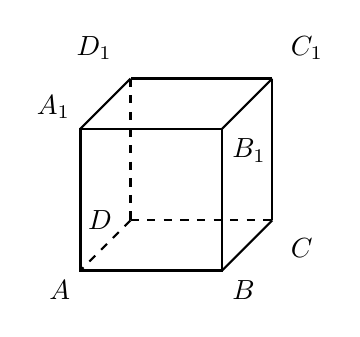
\begin{tikzpicture}[
        scale=0.6,
        % 定义一个样式，用于表示倾斜的深度线
        % x 表示水平分量，y 表示垂直分量。
        % 这里设置了一个45度的倾斜角，并且深度是x和y方向的组合
        z={(-0.3535cm, -0.3535cm)},
        x={(1cm, 0cm)},
        y={(0cm, 1cm)},
        thick % 设置线条为粗体
    ]
    % 定义正方体的边长
    \def\s{3}

    % --- 绘制后方面（隐藏） ---
    % 先定义坐标点
    \coordinate (D) at (0,0,0);
    \coordinate (C) at (\s,0,0);
    \coordinate (D1) at (0,\s,0);
    \coordinate (C1) at (\s,\s,0);
    % 绘制隐藏的边
    \draw (C1) -- (D1);
    \draw (C1) -- (C);
    \draw[dashed] (D1) -- (D);
    \draw[dashed] (D) -- (C);

    % --- 绘制前方面（可见） ---
    % 定义坐标点，z=\s 表示向观察者方向移动 \s 的距离
    \coordinate (A) at (0,0,\s);
    \coordinate (B) at (\s,0,\s);
    \coordinate (A1) at (0,\s,\s);
    \coordinate (B1) at (\s,\s,\s);
    % 绘制可见的正面
    \draw (A) -- (B) -- (B1) -- (A1) -- cycle;

    % --- 连接前后两个面 ---
    \draw[dashed] (D) -- (A); % 这条边被正面遮挡，是虚线
    \draw (C) -- (B);
    \draw (C1) -- (B1);
    \draw (D1) -- (A1);

    % --- 标注顶点 ---
    \node[below left] at (A) {$A$};
    \node[below right] at (B) {$B$};
    \node[below right=3pt] at (C) {$C$};
    \node[left=3pt] at (D) {$D$};
    \node[above left] at (A1) {$A_1$};
    \node[below right] at (B1) {$B_1$};
    \node[above right=3pt] at (C1) {$C_1$};
    \node[above left=3pt] at (D1) {$D_1$};

\end{tikzpicture}